\let\negmedspace\undefined
\let\negthickspace\undefined
\documentclass[journal]{IEEEtran}
\usepackage[a5paper, margin=10mm, onecolumn]{geometry}
%\usepackage{lmodern} % Ensure lmodern is loaded for pdflatex
\usepackage{tfrupee} % Include tfrupee package

\setlength{\headheight}{1cm} % Set the height of the header box
\setlength{\headsep}{0mm}     % Set the distance between the header box and the top of the text

\usepackage{gvv-book}
\usepackage{gvv}
\usepackage{cite}
\usepackage{amsmath,amssymb,amsfonts,amsthm}
\usepackage{algorithmic}
\usepackage{graphicx}
\usepackage{textcomp}
\usepackage{xcolor}
\usepackage{txfonts}
\usepackage{listings}
\usepackage{enumitem}
\usepackage{mathtools}
\usepackage{gensymb}
\usepackage{comment}
\usepackage[breaklinks=true]{hyperref}
\usepackage{tkz-euclide} 
\usepackage{listings}
% \usepackage{gvv}                                        
\def\inputGnumericTable{}                                 
\usepackage[latin1]{inputenc}                                
\usepackage{color}                                            
\usepackage{array}                                            
\usepackage{longtable}                                       
\usepackage{calc}                                             
\usepackage{multirow}                                         
\usepackage{hhline}                                           
\usepackage{ifthen}                                           
\usepackage{lscape}
\usepackage{circuitikz}
\tikzstyle{block} = [rectangle, draw, fill=blue!20, 
    text width=4em, text centered, rounded corners, minimum height=3em]
\tikzstyle{sum} = [draw, fill=blue!10, circle, minimum size=1cm, node distance=1.5cm]
\tikzstyle{input} = [coordinate]
\tikzstyle{output} = [coordinate]


\begin{document}

\bibliographystyle{IEEEtran}
\vspace{3cm}

\title{4.11.4}
\author{EE25BTECH11026-Harsha}
 \maketitle
% \newpage
% \bigskip
{\let\newpage\relax\maketitle}

\renewcommand{\thefigure}{\theenumi}
\renewcommand{\thetable}{\theenumi}
\setlength{\intextsep}{10pt} % Space between text and floats


\numberwithin{equation}{enumi}
\numberwithin{figure}{enumi}
\renewcommand{\thetable}{\theenumi}

\textbf{Question}:\\
Find the equation of the plane which contains the line of intersection of the planes $\vec{r}.\brak{\hat{i}+2\hat{j}+3\hat{k}}-4=0$ and $\vec{r}.\brak{2\hat{i}+\hat{j}-\hat{k}}+5=0$ and which is perpendicular to the plane $\vec{r}.\brak{5\hat{i}+3\hat{j}-6\hat{k}}+8=0$.\\
\solution \\
Let us solve the given question theoretically and then verify the solution computationally.\\
\\
According to the question,\\
\begin{align}
    \vec{n_1}=\myvec{1\\2\\3} \quad \vec{n_2}=\myvec{2\\1\\-1} \quad c_1=4 \quad c_2=-5
\end{align}
The equation of intersection of planes is given by
\begin{align}
    \vec{n_1}^{\top}\vec{x}-c_1+\lambda\brak{\vec{n_2}^{\top}\vec{x}-c_2}=0
\end{align}
\begin{align}
    \implies \brak{\vec{n_1}^{\top}+\lambda\vec{n_2}^{\top}}\vec{x}=c_1+\lambda c_2
\end{align}
Let the direction vector of the plane perpendicular to intersection of planes be $\vec{n_3}$
\begin{align}
    \therefore \brak{\vec{n_1}^{\top}+\lambda\vec{n_2}^{\top}}\vec{n_3}=0
\end{align}
\begin{align}
    \implies \lambda=-\frac{\vec{n_1}^{\top}\vec{n_3}}{\vec{n_2}^{\top}\vec{n_3}}
\end{align}
\begin{align}
    \therefore \lambda=-\frac{\myvec{1&&2&&3}\myvec{5\\3\\-6}}{\myvec{2&&1&&-1}\myvec{5\\3\\-6}}=\frac{7}{19}
\end{align}
\begin{align}
    \implies \text{equation of the plane\,:\;} \myvec{33&&45&&50}\vec{x}=41
\end{align}

\newpage
\vspace*{0.25cm}

From the figure, it is clearly verified that the theoretical solution matches with the computational solution.\\
\begin{figure}[H]
    \centering
    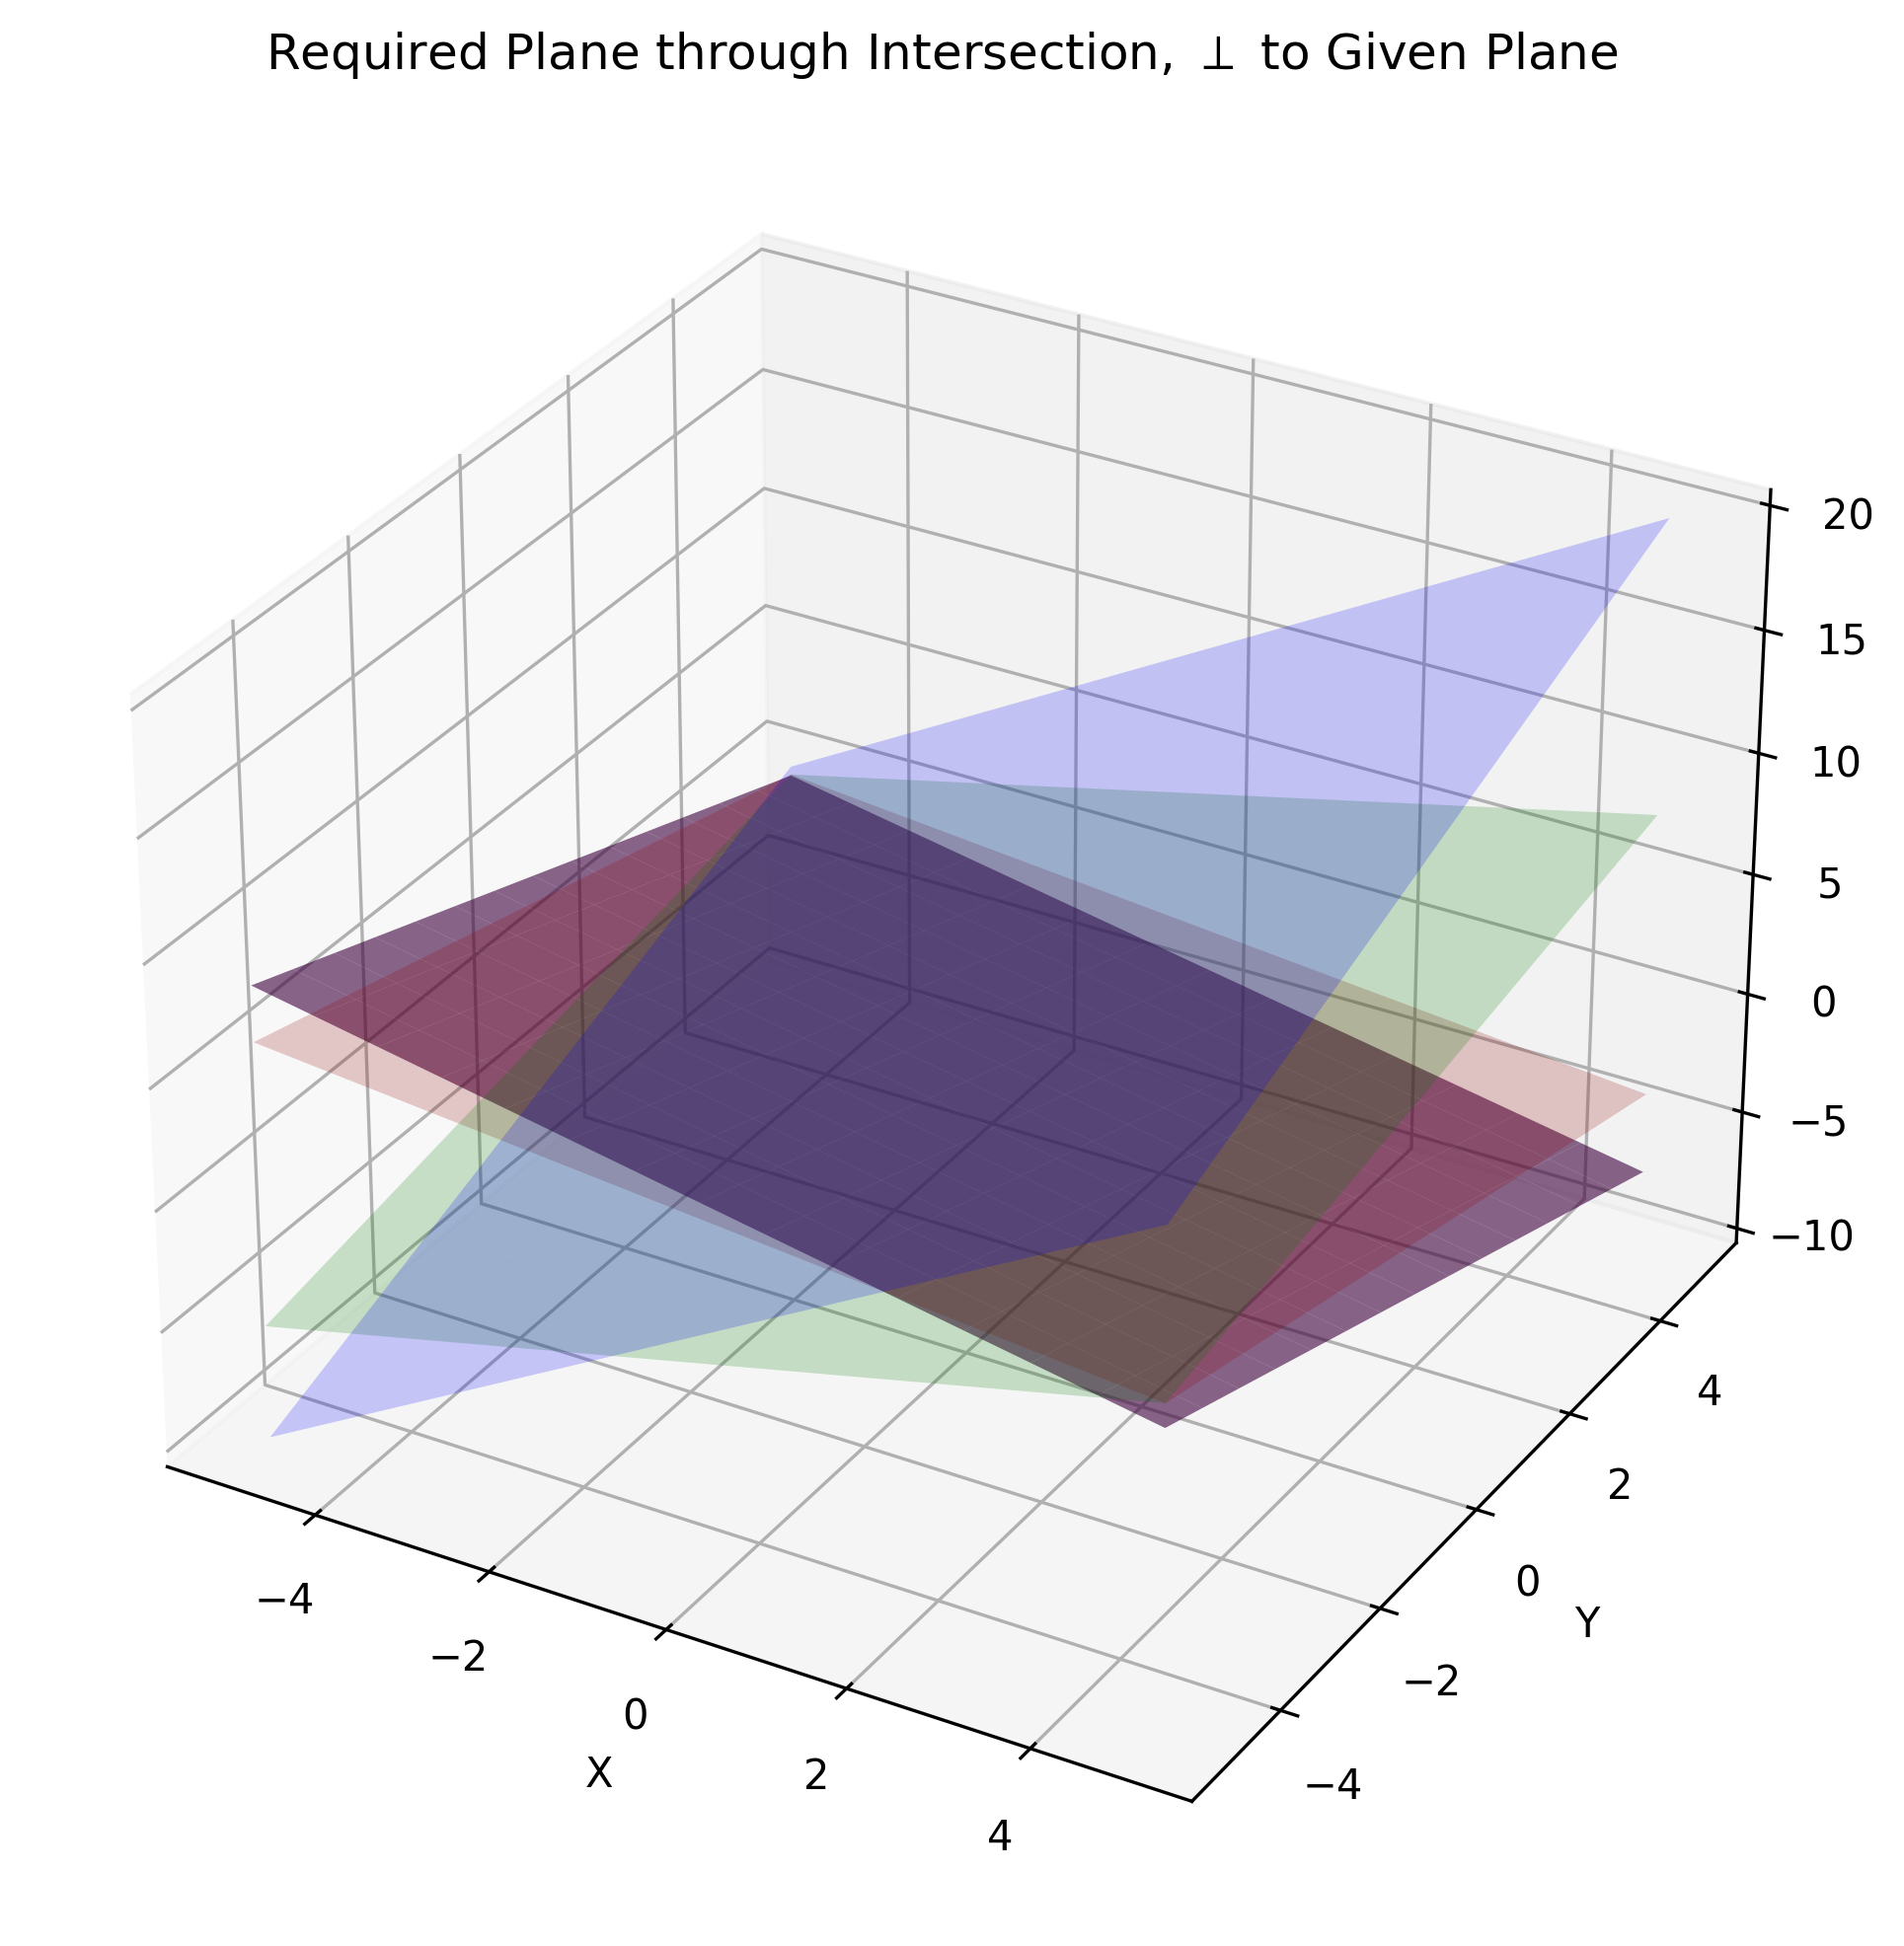
\includegraphics[width=0.8\columnwidth]{figs/Figure_1.png}
    \label{fig:1}
\end{figure}


\end{document}
